\documentclass[conference]{IEEEtran}

% Core
\usepackage{cite}
\usepackage{amsmath,amssymb,amsfonts}
\usepackage{graphicx}
\usepackage{booktabs}
\usepackage{makecell}
\renewcommand\theadfont{\normalsize\bfseries}
\usepackage{array}
\usepackage{multirow}
\usepackage{siunitx}
\usepackage{bm}
\usepackage{url}
\usepackage{hyperref}
\usepackage{xcolor}
\usepackage{algorithm}
\usepackage{algorithmic}

% Floats & subfigures
\usepackage{subcaption}
\usepackage{dblfloatfix}
\usepackage{tikz}
\usetikzlibrary{arrows.meta, positioning, fit, backgrounds, calc}

\newcommand{\TODO}[1]{\textcolor{red}{\textbf{TODO:} #1}}

\title{Clearing Dense Log Piles with Imitation-Bootstrapped Reinforcement Learning}

\author{
Anonymous Authors
}
\begin{document}
\maketitle

\begin{abstract}
Clearing a dense pile of logs by sequential grasping is a contact-rich manipulation problem. The scene contains hundreds of rigid bodies in frictional contact, each grasp reshapes the pile, and effective strategies span long horizons.
We study this problem in simulation for a forestry log loader that must clear piles of 200 logs using only depth-derived point clouds requiring no semantic segmentation.
From-scratch reinforcement learning (RL) fails to discover effective clearing strategies regardless of observation type.
Our framework first trains a PointNet-based policy via behavior cloning (BC) on demonstrations from a privileged-state heuristic, then fine-tunes with RL using an asymmetric actor-critic.
BC provides the full-trajectory exploration curriculum that RL alone cannot discover, while RL optimizes per-grasp quality beyond what the demonstrator achieves.
The resulting policy maintains expert-level clearing ($98.2$\%) while improving grasp stability by $15$\% over the BC initialization, using only depth-derived point clouds.
\end{abstract}

\begin{IEEEkeywords}
robot learning, multi-object grasping from dense clutter, behavior cloning, reinforcement learning fine-tuning, contact-rich simulation
\end{IEEEkeywords}

\section{Introduction}
Forestry operations increasingly seek autonomy for heavy machinery to improve safety and productivity~\cite{lindroos2015forestry}.
A key subtask is log-pile clearing: repeatedly grasping multiple logs from a rack or pile and removing them.
This setting is challenging because (i) the scene is densely cluttered with hundreds of rigid-body logs in frictional contact, (ii) each grasp disturbs the pile through contact cascades, continuously reshaping the configuration for subsequent attempts, and (iii) no two pile configurations are alike, so a targeting strategy must be robust to diverse arrangements.

\begin{figure}[b]
\centering
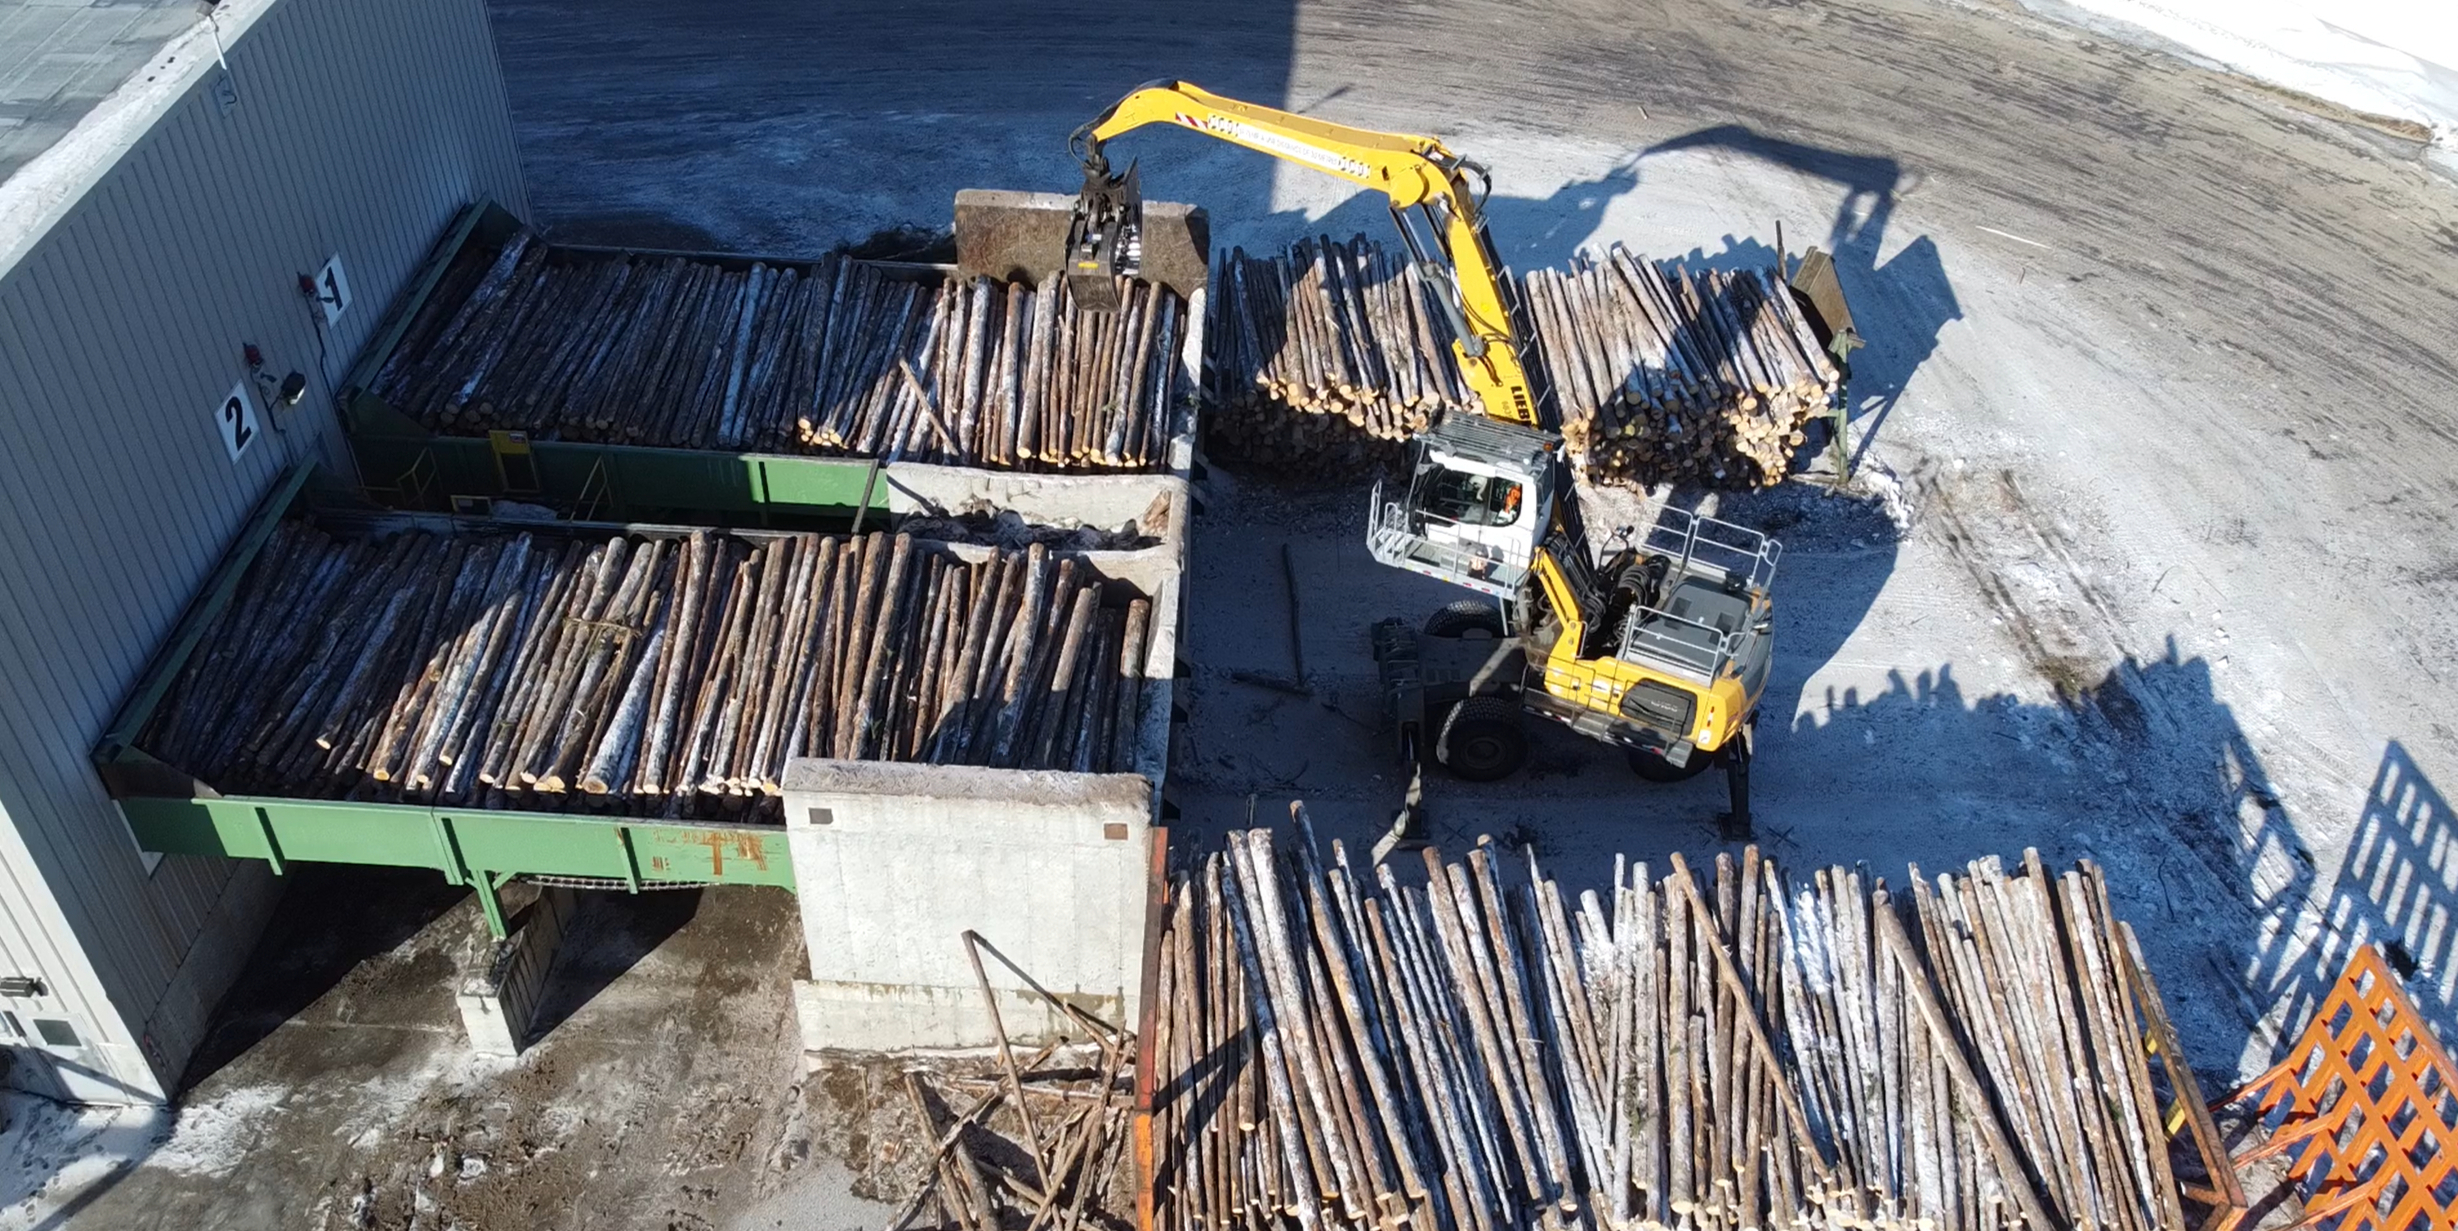
\includegraphics[width=\columnwidth]{mill.pdf}
\caption{A log loader clearing piles at a millyard infeed deck. Our work targets autonomous grasp selection for this task using only depth-derived point clouds.}
\label{fig:mill}
\end{figure}

We address grasp target selection: given a raw point cloud from a stereo depth camera, where should the crane grasp to clear the pile efficiently?
We separate this targeting decision from low-level execution via a grasp-and-remove simulator in Isaac Lab~\cite{mittal2023orbit}, where each step is one complete pick attempt and grasped logs are removed rather than deposited.
Existing work addresses small-scale settings (single-log pick-and-place, groupings of 2--7 logs, or grasp prediction without sequential clearing); we scale to pile-level clearing with dense frictional contact among hundreds of logs.

Dense pile clearing poses a difficult exploration problem for RL: reward is sparse across long episodes, and from-scratch RL stalls at roughly 53\% clearing regardless of observation type.
Our approach trains a policy via behavior cloning (BC) on demonstrations from a privileged-state heuristic, then fine-tunes with RL.
The demonstration data spans the complete clearing trajectory, providing the distributional coverage that RL cannot acquire through its own exploration.

Our main contributions are:
\begin{itemize}
    \item A BC$\to$RL pipeline where a PointNet encoder, pretrained via BC on heuristic demonstrations from raw point clouds, is frozen during RL while the policy head is updated with an asymmetric actor-critic~\cite{pinto2018asymmetric}. This prevents catastrophic forgetting while letting RL optimize per-grasp execution; the resulting policy surpasses the expert in grasp stability using depth alone.
    \item A grasp-and-remove crane environment in Isaac Lab for dense pile clearing (200 logs) with a fixed FSM isolating targeting from execution.
    \item A four-method comparison: (a) from-scratch RL fails regardless of observation type, (b) BC achieves near-expert clearing from raw point clouds, (c) BC+RL improves stability by 15\% while maintaining clearing.
\end{itemize}

\section{Related Work}

\subsection{Grasping in Clutter}
Learning-based grasping has progressed from isolated objects to cluttered scenes, with deep networks predicting grasp poses from depth~\cite{morrison2018closing, kumra2017robotic} and synthetic data enabling robust planning~\cite{mahler2017dexnet}.
Sequential decluttering has been studied in bin picking~\cite{mahler2017sequential, zeng2018learning} and extended to forestry log loading~\cite{wallin2024multilog}.
These works typically involve heterogeneous objects in loose arrangements with precision grasps isolating single targets.
Our setting differs: we perform power grasps from dense piles of uniformly cylindrical logs in extensive frictional contact, where each multi-log grasp disturbs the pile, reshaping subsequent configurations.
For 3D perception of unordered point sets, PointNet~\cite{qi2017pointnet} provides a natural encoder.

\subsection{Learning for Log Grasping and Forestry Crane Control}
Existing learning-based approaches to log grasping address smaller-scale settings than the one considered here.
For grasp prediction, methods range from RL with visual servoing for 2--5 log groupings~\cite{wallin2024multilog}, to CNN-based grasp pose prediction from synthetic RGB-D for clusters of up to 7 logs~\cite{falldin2025synthesizing, ayoub2023grasp}.
For crane control, recent work benchmarks RL velocity controllers for single-log grasping in simulation~\cite{vu2025autonomous, kurinov2025reinforcement}, and dynamic programming has been applied to anti-sway trajectory design~\cite{jebellat2025designing}.
These works address individual subtasks but none tackle sequential clearing of a dense pile at the scale considered here.

\section{Task Formulation}
\subsection{Grasp-and-Remove Formulation}
\label{sec:formulation}
Each environment step corresponds to a complete grasp attempt: a policy selects a grasp target, the FSM executes the approach, close, and lift, and grasped logs are removed from the scene.
This formulation is shared by all methods (heuristic, BC, RL, and BC+RL).
The state $s_t \in \mathcal{S}$ is the current pile configuration (observed via point cloud or privileged poses; Section~\ref{sec:obs}).
A grasp target is defined by the tuple
\begin{equation}
    \mathbf{g} = (x,\, y,\, z,\, \psi),
\end{equation}
where $(x, y, z)$ is the grapple position in the crane base frame and $\psi$ is the grapple yaw angle about the vertical axis.
Because a cylindrical log at yaw $\psi$ is identical to the same log at $\psi + \pi$, the policy represents $\psi$ via the $\pi$-periodic encoding $(\cos 2\psi, \sin 2\psi)$~\cite{morrison2018closing}, giving a 5D action $a_t \in \mathcal{A} \subset \mathbb{R}^5$ (Section~\ref{sec:actions}).
The transition $T(s_{t+1}|s_t, a_t)$ is determined by the physics simulation and FSM execution.
After each grasp attempt, an outcome evaluation measures the number of logs grasped, grapple--log alignment, and grapple stability (Section~\ref{sec:outcome}).
For RL training, this outcome is used as a scalar reward $r_t = R(s_t, a_t)$, and the full structure is treated as an episodic Markov decision process $(\mathcal{S}, \mathcal{A}, T, R, \gamma)$ with discount factor $\gamma$, where a policy $\pi$ maximizes the expected discounted return over a horizon of $H$ grasp attempts:
\begin{equation}
    \max_\pi \; \mathbb{E}_\pi \!\left[\sum_{t=0}^{H-1} \gamma^t \, r_t \right].
\end{equation}
An episode terminates when no logs remain or after a fixed horizon of $H=30$ grasp attempts.
The horizon is chosen to exceed the minimum needed: the grapple can hold up to 20 logs per grasp, and the heuristic clears 200-log piles in approximately 20 attempts, so $H=30$ provides a 50\% margin while keeping episodes tractable.
Logs leave the rack by grasping or by being knocked out of bounds (Section~\ref{sec:outcome}); only intentionally grasped logs count toward the clearing rate (Section~\ref{sec:metrics}).


\subsection{Observations}
\label{sec:obs}
A depth camera mounted above the rack (simulated with parameters matching the Stereolabs ZED~X\footnote{\url{https://www.stereolabs.com/products/zed-x}}) renders the scene at each step.
The observation pipeline (Fig.~\ref{fig:pcd_pipeline}) back-projects valid depth pixels to 3D points, transforms them into the crane base frame, and applies Farthest Point Sampling (FPS) to produce a fixed-size observation $o_t = \mathrm{FPS}(\mathcal{P}_b,\; N_p) \in \mathbb{R}^{1024 \times 3}$.
No semantic segmentation is applied: the raw point cloud includes all visible surfaces (logs, rack, ground), and the PointNet encoder must learn to attend to task-relevant geometry.
We compare raw and segmented point clouds in Section~\ref{sec:results}.

As an ablation, we evaluate policies observing privileged per-object state: the top-$K\!=\!32$ log poses sorted by height, each as $(x,y,z,\psi)$ in the crane base frame ($4K = 128$D vector, padded with $-1$ for removed logs).
This isolates the perception gap from the learning algorithm.

\subsection{Actions and Workspace Scaling}
\label{sec:actions}
The policy outputs a 5D vector $\tilde{a}_t \in \mathbb{R}^5$ (before squashing).
The first three components encode position and the remaining two encode grapple yaw via a cosine--sine pair.

Each position component is squashed via the hyperbolic tangent $\tanh$ and then linearly mapped to the per-environment workspace bounds to produce the target coordinate $p_i$:
\begin{equation}
    p_i = \frac{(\tanh \tilde{a}_i + 1)}{2}(b_i^{\max} - b_i^{\min}) + b_i^{\min}, \quad i \in \{x,y,z\},
\end{equation}
where $b_i^{\min}, b_i^{\max}$ are the rack-aligned workspace limits for each axis.
These bounds are derived from the rack geometry with margins along each axis.
The resulting workspace is approximately $2.0 \times 5.2 \times 1.0$\,m in the crane base frame.
Logs that drift outside these bounds during a grasp (e.g., knocked off the rack) are removed before the next step and counted separately (Section~\ref{sec:outcome}).

The remaining two components encode grapple yaw via a $\pi$-periodic cosine-sine pair~\cite{morrison2018closing}, exploiting the symmetry that a cylindrical log at yaw $\psi$ is identical to one at $\psi + \pi$:
\begin{equation}
    \psi = \tfrac{1}{2}\,\mathrm{atan2}\!\big(\tanh \tilde{a}_5,\;\tanh \tilde{a}_4\big) \;\in \big[-\tfrac{\pi}{2},\;\tfrac{\pi}{2}\big].
\end{equation}
Expert targets for BC are encoded identically (positions via $\mathrm{arctanh}$, yaw as $\cos 2\psi, \sin 2\psi$).

\section{Environment and Controller}
\subsection{Low-level Execution FSM}
All methods share the same fixed FSM controller, which runs at the control rate (60\,Hz, i.e., 120\,Hz physics with $2\times$ decimation) inside each environment step.
Given a grasp target $(x,y,z,\psi)$, produced by the heuristic (Section~\ref{sec:expert}) or a learned policy (BC or RL), the FSM executes a complete grasp cycle.

The crane arm has four actuated joints (basemast, boom, stick, and telescope) followed by a two-link passive chain that suspends the grapple from the telescope tip via unactuated revolute joints with low stiffness and damping.
Below the passive chain, a yaw joint rotates the grapple about the vertical axis and two gripper joints control the jaw opening.
Because the grapple hangs $\sim$0.4\,m below the IK target link, all grasp targets are offset vertically and the FSM waits for pendulum oscillations to damp before advancing each phase.

The FSM executes a five-phase grasp cycle: \texttt{HOVER} (move above the target with 2.5\,m clearance), \texttt{ALIGN} (rotate to target yaw $\psi$), \texttt{DESCEND} (lower at reduced speed to minimize pile disturbance), \texttt{CLOSE} (close jaws incrementally), and \texttt{LIFT} (raise to hover height and evaluate grasp outcome per Section~\ref{sec:outcome}; grasped logs are removed and the cycle repeats).
The arm is controlled via Isaac Lab's Differential IK controller~\cite{mittal2023orbit}; the grapple yaw and jaws use independent PD controllers.

\subsection{Outcome Evaluation}
\label{sec:outcome}
After the \texttt{LIFT} phase, grasp outcome is evaluated by measuring proximity and orientation of logs relative to the grapple body (Fig.~\ref{fig:grasp_geometry}).
\textbf{Logs grasped} ($g$): active logs whose centers lie within a proximity radius (1.5\,m) of the grapple.
\textbf{Alignment} ($\alpha$): parallelism between the grapple jaw axis $\hat{y}_g$ and each log's length axis $\hat{y}_{\ell_i}$, raised to the 8th power for sharp misalignment penalty:
\begin{equation}
    \alpha_i = \big(\hat{y}_g^\top \hat{y}_{\ell_i}\big)^{8}, \qquad \alpha = \frac{1}{g}\sum_{i=1}^{g} \alpha_i \;\in [0,1].
\end{equation}
\textbf{Stability} ($\varsigma$): grapple levelness after lifting, raised to the 4th power:
\begin{equation}
    \varsigma = \big(\max(0,\;\hat{z}_g^\top \hat{z}_w)\big)^{4} \;\in [0,1].
\end{equation}
\textbf{Grasp quality} is defined as $q = \alpha \cdot \varsigma \in [0,1]$.
Grasped logs are removed from the scene; logs knocked out of bounds are removed separately and excluded from $g$.

\begin{figure}[t]
\centering

\includegraphics[width=\columnwidth]{outcomes.png}

\caption{Coordinate frames used to compute alignment ($\alpha$) and stability ($\varsigma$). The alignment score measures parallelism between the grapple jaw axis $\hat{y}_g$ and the log length axis $\hat{y}_\ell$; stability measures the grapple's levelness via $\hat{z}_g^\top \hat{z}_w$.}
\label{fig:grasp_geometry}
\end{figure}

The environment runs on PhysX GPU dynamics in Isaac Lab.
Log and contact parameters (Table~\ref{tab:sim_params}) are based on representative forestry logs and published friction coefficients~\cite{avallone2006marks}, with conservative contact modeling to reduce interpenetration.


\begin{table}[t]
\centering
\caption{Simulation and controller parameters.}
\label{tab:sim_params}
\setlength{\tabcolsep}{2pt}
\footnotesize
\begin{tabular}{@{}lr@{\hskip 8pt}lr@{}}
\toprule
\multicolumn{2}{l}{\textit{Simulation \& FSM}} & \multicolumn{2}{l}{\textit{Actuator gains} ($k_p/k_d$)} \\[2pt]
Physics $\Delta t$ & $1/120$\,s & Main arm & $10^{6}/10^{5}$ \\
Control dec. & $2\times$ (60\,Hz) & Passive chain & $300/500$ \\
Hover clearance & 2.5\,m & Grapple yaw & $5\!\times\!10^{4}/2\!\times\!10^{4}$ \\
Pos.\ tol.\ (up/bg) & 0.10/0.25\,m & Grapple tongs & $0/500$ \\
Dwell / timeout & 30 / 100 steps & IK arm $k_p/k_d$ & $4.0/1.2$ \\
\addlinespace[3pt]
\multicolumn{2}{l}{\textit{Log properties}} & \multicolumn{2}{l}{\textit{Crane link masses}} \\[2pt]
Diameter / length & 0.3 / 3.0\,m & Mast / Boom / Stick & 290/172/70\,kg \\
Mass & 15\,kg & Telescope / Upper & 25/9\,kg \\
$\mu_s / \mu_k$ & 0.62 / 0.48 & & \\
Ang.\ damping & 0.05 & & \\
Contact / rest off. & 0.02 / 0.0\,m & & \\
Max depenetration & 3.0\,m/s & & \\
\bottomrule
\end{tabular}
\end{table}

\section{Baseline and Learned Policies}

\subsection{Heuristic Expert}
\label{sec:expert}
The heuristic expert serves as both a baseline and the demonstration source for BC.
It has access to privileged state (all active log poses from the physics engine) and uses a top-of-pile targeting strategy: at each pick cycle, it selects the topmost log ($\max z$), transforms its position into the crane base frame as the $(x,y,z)$ target, and aligns the grapple yaw to the log's length axis.
Because of the $\pi$-symmetry, both yaw orientations are evaluated and the one requiring minimal joint rotation is chosen.
Yaw alignment is recomputed in closed loop during the \texttt{ALIGN} phase.

This greedy strategy is effective for dense piles, where the topmost log is typically the most accessible.
In the endgame, when scattered logs remain, the strategy is no longer clearly optimal, but the expert still achieves strong performance across all metrics (Table~\ref{tab:results}).

\subsection{Behavior Cloning}
\label{sec:bc}
We train a BC policy~\cite{pomerleau1988alvinn} on successful expert grasps $(o_t, a_t)$, where actions are in the pre-squashing space (Section~\ref{sec:actions}).
The policy uses a PointNet encoder~\cite{qi2017pointnet}: a per-point MLP ($3 \!\to\! 64 \!\to\! 128 \!\to\! 256$, BN, ELU) followed by symmetric max-pooling to produce a global feature $\mathbf{z} \in \mathbb{R}^{256}$, then an actor MLP ($256 \!\to\! 128 \!\to\! 64 \!\to\! 5$) maps to the action.
Table~\ref{tab:architecture} summarizes all architectures.

\begin{table}[t]
\centering
\caption{Network architectures. All hidden layers use ELU activations. The PointNet encoder applies batch normalization. All policies output 5D actions: $(x,y,z,\cos 2\psi,\sin 2\psi)$.}
\label{tab:architecture}
\setlength{\tabcolsep}{3pt}
\begin{tabular}{@{}lp{2.4cm}p{2.4cm}p{2.0cm}@{}}
\toprule
& \textbf{BC / RL (PCD)} & \textbf{BC+RL (PCD)} & \textbf{RL (Pose)} \\
\midrule
Encoder
  & PointNet: $3\!\to\!64\!\to\!128\!\to\!256$, BN, max-pool
  & Same (frozen, init from BC)
  & MLP: $128\!\to\!256\!\to\!128\!\to\!64$ \\[3pt]
Actor
  & $256\!\to\!128\!\to\!64\!\to\!5$
  & Same (init from BC)
  & Shared enc $\to$ $64\!\to\!5$ \\[3pt]
Critic
  & PointNet + MLP head
  & MLP: $128\!\to\!256\!\to\!128\!\to\!1$ (state)
  & MLP: $256\!\to\!128\!\to\!64\!\to\!1$ \\
\bottomrule
\end{tabular}
\end{table}

The BC objective minimizes MSE between predicted and expert actions over $\sim$20{,}700 successful grasps (85/15 train/val split):
\begin{equation}
    \mathcal{L}_{\text{BC}} = \frac{1}{|\mathcal{D}|}\sum_{(o,a^*)\in\mathcal{D}} \left\| \mu_\theta(\mathbf{z}) - a^* \right\|^2.
\end{equation}
We use dropout (0.2), AdamW~\cite{loshchilov2019adamw} ($\text{lr}=10^{-4}$, weight decay $10^{-4}$), and ReduceLROnPlateau scheduling with early stopping.

\subsection{Reinforcement Learning}
\label{sec:rl}
We train policies with PPO~\cite{schulman2017ppo} using RSL-RL~\cite{rudin2022learning}.
PPO optimizes a stochastic Gaussian policy $\pi_\theta(a \mid s) = \mathcal{N}\!\big(\mu_\theta(s),\;\mathrm{diag}(\bm{\sigma}^2)\big)$,
where $\bm{\sigma}$ is a learnable standard deviation vector initialized to $\sigma_0$.
A separate critic estimates the state-value function $V_\phi(s)$; advantages are computed via GAE~\cite{schulman2017ppo}.
The actor uses the same PointNet encoder and MLP as BC; the critic uses an independent encoder with its own MLP head (Table~\ref{tab:architecture}).
Key hyperparameters: $\sigma_0 = 1.0$, $\epsilon=0.2$, entropy coefficient $0.01$, learning rate $3\times10^{-4}$ with adaptive KL scheduling, GAE ($\lambda=0.95$, $\gamma = 0.99$), 4 steps per environment per iteration, 5 epochs with 4 mini-batches.
The outcome components from Section~\ref{sec:outcome} define the reward:
\label{eq:reward}
\begin{equation}
r = g \cdot \alpha \cdot \varsigma = g \cdot q,
\end{equation}
for successful grasps ($g > 0$), and $r = -1$ for failures.
The reward is entirely per-grasp; global clearing must emerge from the targeting strategy.

\begin{figure}[t]
\centering
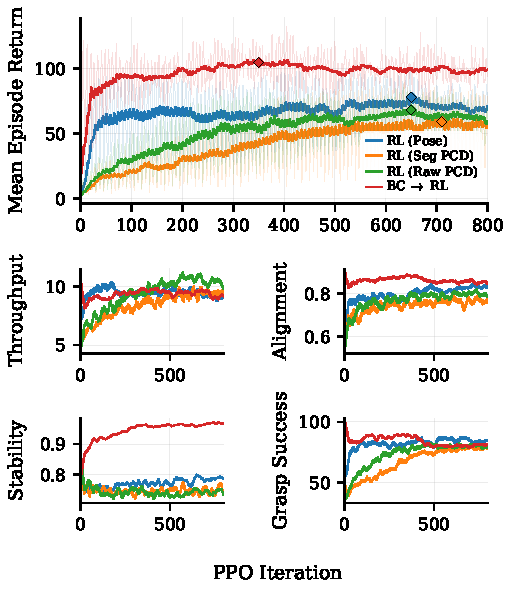
\includegraphics[width=\columnwidth]{reward_curves.pdf}
\caption{PPO training curves (mean episode return vs.\ iteration, 20-iteration rolling average). Diamond markers indicate the checkpoint selected for evaluation. All from-scratch RL variants improve per-grasp reward but fail to achieve full clearing. BC$\to$RL reaches the highest return while maintaining near-complete clearing; performance degrades after $\sim$500 iterations, motivating early stopping.}
\label{fig:reward_curves}
\end{figure}

\subsection{BC-Initialized RL Fine-Tuning}
\label{sec:bcrl}
We initialize a PPO agent from the trained BC policy and fine-tune with on-policy experience~\cite{rajeswaran2018learning, nair2018overcoming}.
The actor weights are loaded from BC; the critic is initialized randomly.
We use an \emph{asymmetric actor-critic}~\cite{pinto2018asymmetric}: the actor observes the raw point cloud, while the critic receives the privileged 128D pose state vector.

The BC-trained PointNet encoder is frozen during RL.
Since the state-based critic cannot propagate gradients through the encoder, an unfrozen encoder drifts without constraint, causing training collapse (Fig.~\ref{fig:bcrl_ablation}).
The only other change from Section~\ref{sec:rl} is reduced initial noise $\sigma_0 = 0.05$ (vs.\ $1.0$), limiting exploration to small perturbations around the BC mean.

\begin{figure*}[t]
\centering
\resizebox{0.92\textwidth}{!}{%
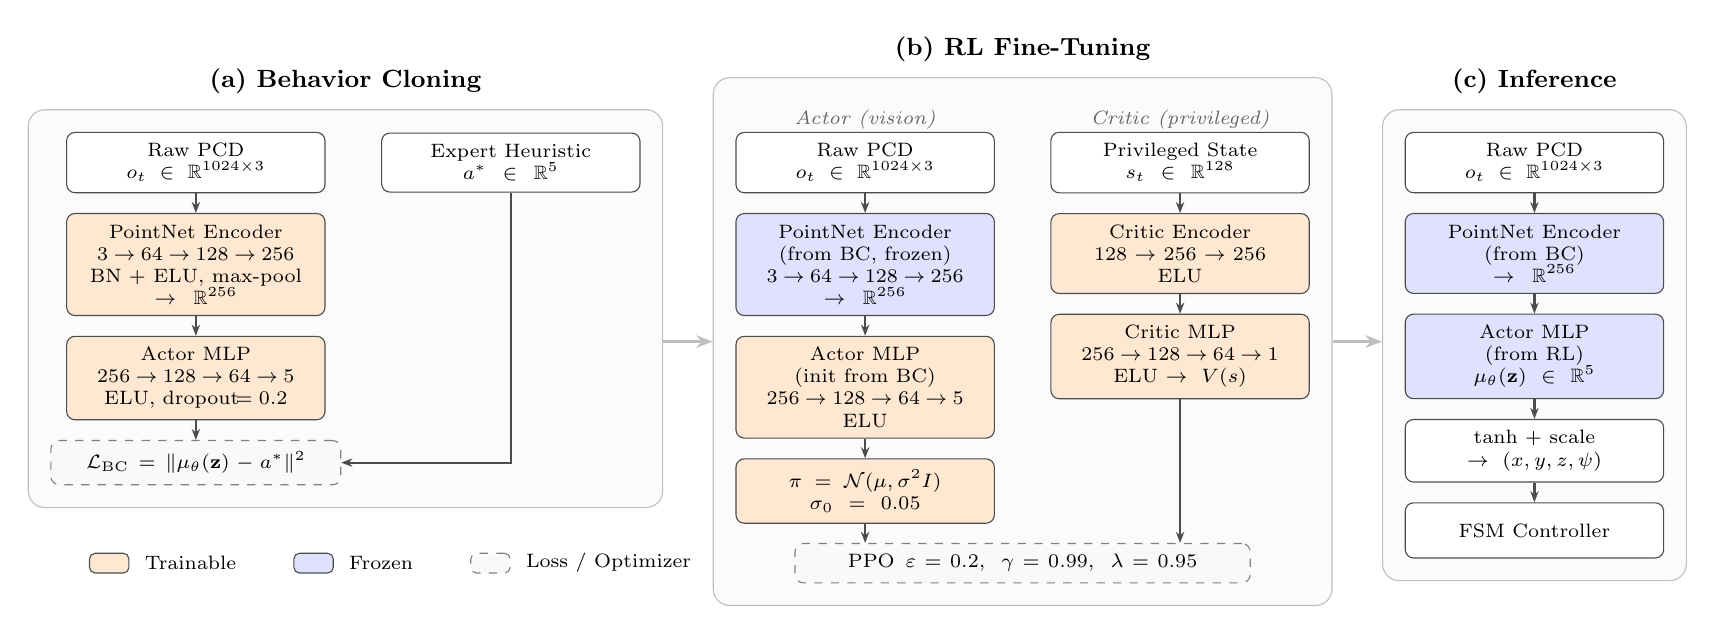
\begin{tikzpicture}[
  block/.style={rectangle, rounded corners=3pt, draw=black!70,
    text width=3.0cm, minimum height=0.7cm, align=center,
    font=\scriptsize, inner sep=4pt},
  frozen/.style={block, fill=blue!12},
  trainable/.style={block, fill=orange!18},
  io/.style={block, fill=white},
  lossnode/.style={rectangle, rounded corners=3pt, draw=black!50, dashed,
    text width=3.4cm, align=center, font=\scriptsize, inner sep=4pt, fill=gray!5},
  wideloss/.style={lossnode, text width=5.5cm},
  arr/.style={-{Stealth[length=4pt]}, thick, black!70},
  panelbg/.style={rectangle, rounded corners=6pt, draw=gray!50,
    fill=gray!3, inner sep=8pt},
  ptitle/.style={font=\small\bfseries},
  collabel/.style={font=\scriptsize\itshape, text=black!60},
]
% ====== PANEL (a): BEHAVIOR CLONING ======
\node[io] (a_pcd) at (0, 0)
  {Raw PCD\\$o_t \in \mathbb{R}^{1024\times3}$};
\node[io] (a_expert) at (4, 0)
  {Expert Heuristic\\$a^{*} \in \mathbb{R}^{5}$};
\node[trainable, below=0.25cm of a_pcd] (a_enc)
  {PointNet Encoder\\$3\!\to\!64\!\to\!128\!\to\!256$\\BN + ELU, max-pool\\$\to\mathbb{R}^{256}$};
\node[trainable, below=0.25cm of a_enc] (a_mlp)
  {Actor MLP\\$256\!\to\!128\!\to\!64\!\to\!5$\\ELU, dropout$\!=\!0.2$};
\node[lossnode, below=0.25cm of a_mlp] (a_loss)
  {$\mathcal{L}_{\text{BC}} = \lVert\mu_\theta(\mathbf{z}) - a^{*}\rVert^{2}$};
\draw[arr] (a_pcd) -- (a_enc);
\draw[arr] (a_enc) -- (a_mlp);
\draw[arr] (a_mlp) -- (a_loss);
\draw[arr] (a_expert.south) |- (a_loss.east);
%
% ====== PANEL (b): RL FINE-TUNING ======
\node[collabel] (b_alabel) at (8.5, 0.55) {Actor (vision)};
\node[collabel] (b_clabel) at (12.5, 0.55) {Critic (privileged)};
% Actor column
\node[io] (b_pcd) at (8.5, 0) {Raw PCD\\$o_t \in \mathbb{R}^{1024\times3}$};
\node[frozen, below=0.25cm of b_pcd] (b_enc)
  {PointNet Encoder\\(from BC, frozen)\\$3\!\to\!64\!\to\!128\!\to\!256$\\$\to\mathbb{R}^{256}$};
\node[trainable, below=0.25cm of b_enc] (b_actor)
  {Actor MLP\\(init from BC)\\$256\!\to\!128\!\to\!64\!\to\!5$\\ELU};
\node[trainable, below=0.25cm of b_actor] (b_policy)
  {$\pi = \mathcal{N}(\mu, \sigma^{2} I)$\\$\sigma_0 = 0.05$};
% Critic column
\node[io] (b_state) at (12.5, 0)
  {Privileged State\\$s_t \in \mathbb{R}^{128}$};
\node[trainable, below=0.25cm of b_state] (b_cenc)
  {Critic Encoder\\$128\!\to\!256\!\to\!256$\\ELU};
\node[trainable, below=0.25cm of b_cenc] (b_cmlp)
  {Critic MLP\\$256\!\to\!128\!\to\!64\!\to\!1$\\ELU $\to V(s)$};
% PPO node spanning both columns (anchored below deepest column, centered)
\path (b_policy.south) ++(0,-0.5) coordinate (ppo_y);
\path (b_pcd.center) -- (b_state.center) coordinate[midway] (ppo_x);
\node[wideloss] (b_ppo) at (ppo_y -| ppo_x)
  {PPO\enspace $\varepsilon\!=\!0.2,\;\gamma\!=\!0.99,\;\lambda\!=\!0.95$};
\draw[arr] (b_pcd) -- (b_enc);
\draw[arr] (b_enc) -- (b_actor);
\draw[arr] (b_actor) -- (b_policy);
\draw[arr] (b_state) -- (b_cenc);
\draw[arr] (b_cenc) -- (b_cmlp);
\draw[arr] (b_policy.south) -- (b_policy |- b_ppo.north);
\draw[arr] (b_cmlp.south) -- (b_cmlp |- b_ppo.north);
%
% ====== PANEL (c): INFERENCE ======
\node[io] (c_pcd) at (17, 0) {Raw PCD\\$o_t \in \mathbb{R}^{1024\times3}$};
\node[frozen, below=0.25cm of c_pcd] (c_enc)
  {PointNet Encoder\\(from BC)\\$\to\mathbb{R}^{256}$};
\node[frozen, below=0.25cm of c_enc] (c_actor)
  {Actor MLP\\(from RL)\\$\mu_\theta(\mathbf{z}) \in \mathbb{R}^{5}$};
\node[io, below=0.25cm of c_actor] (c_scale)
  {tanh + scale\\$\to(x,y,z,\psi)$};
\node[io, below=0.25cm of c_scale] (c_fsm) {FSM Controller};
\draw[arr] (c_pcd) -- (c_enc);
\draw[arr] (c_enc) -- (c_actor);
\draw[arr] (c_actor) -- (c_scale);
\draw[arr] (c_scale) -- (c_fsm);
%
% ====== PANEL BACKGROUNDS (consolidated, natural height per panel) ======
\begin{scope}[on background layer]
  \node[panelbg, fit=(a_pcd)(a_expert)(a_enc)(a_mlp)(a_loss)] (bg_a) {};
  \node[panelbg, fit=(b_alabel)(b_clabel)(b_pcd)(b_enc)(b_actor)(b_policy)(b_state)(b_cenc)(b_cmlp)(b_ppo)] (bg_b) {};
  \node[panelbg, fit=(c_pcd)(c_enc)(c_actor)(c_scale)(c_fsm)] (bg_c) {};
\end{scope}
\node[ptitle, above=2pt of bg_a.north] {(a) Behavior Cloning};
\node[ptitle, above=2pt of bg_b.north] {(b) RL Fine-Tuning};
\node[ptitle, above=2pt of bg_c.north] {(c) Inference};
%
% ====== STAGE ARROWS (level, pinned to panel b midpoint) ======
\draw[-{Stealth[length=6pt]}, very thick, gray!50]
  (bg_a.east |- bg_b.west) -- (bg_b.west);
\draw[-{Stealth[length=6pt]}, very thick, gray!50]
  (bg_b.east) -- (bg_c.west |- bg_b.east);
%
% ====== LEGEND ======
\coordinate (leg_start) at ($(bg_a.center |- b_ppo) + (-3.0, 0)$);
\node[rectangle, rounded corners=2pt, draw=black!70, fill=orange!18,
  minimum width=0.5cm, minimum height=0.25cm] (leg_t) at (leg_start) {};
\node[font=\scriptsize, right=2pt of leg_t] (leg_tl) {Trainable};
\node[rectangle, rounded corners=2pt, draw=black!70, fill=blue!12,
  minimum width=0.5cm, minimum height=0.25cm, right=0.6cm of leg_tl] (leg_f) {};
\node[font=\scriptsize, right=2pt of leg_f] (leg_fl) {Frozen};
\node[rectangle, rounded corners=2pt, draw=black!50, dashed, fill=gray!5,
  minimum width=0.5cm, minimum height=0.25cm, right=0.6cm of leg_fl] (leg_l) {};
\node[font=\scriptsize, right=2pt of leg_l] {Loss / Optimizer};
\end{tikzpicture}%
}% end resizebox
\caption{The BC$\to$RL pipeline. (a)~The PointNet encoder and actor MLP are trained end-to-end on expert demonstrations with MSE loss. (b)~The encoder is frozen and the actor MLP is fine-tuned with PPO alongside a state-based asymmetric critic. (c)~At inference the critic is discarded; the encoder and actor run deterministically.}
\label{fig:bcrl_pipeline}
\end{figure*}
Higher noise causes gradual degradation ($\sigma_0 = 0.1$) or rapid collapse ($\sigma_0 = 0.3$), as shown in Fig.~\ref{fig:bcrl_ablation}.

\begin{figure*}[t]                                                                                                                    
\centering                         
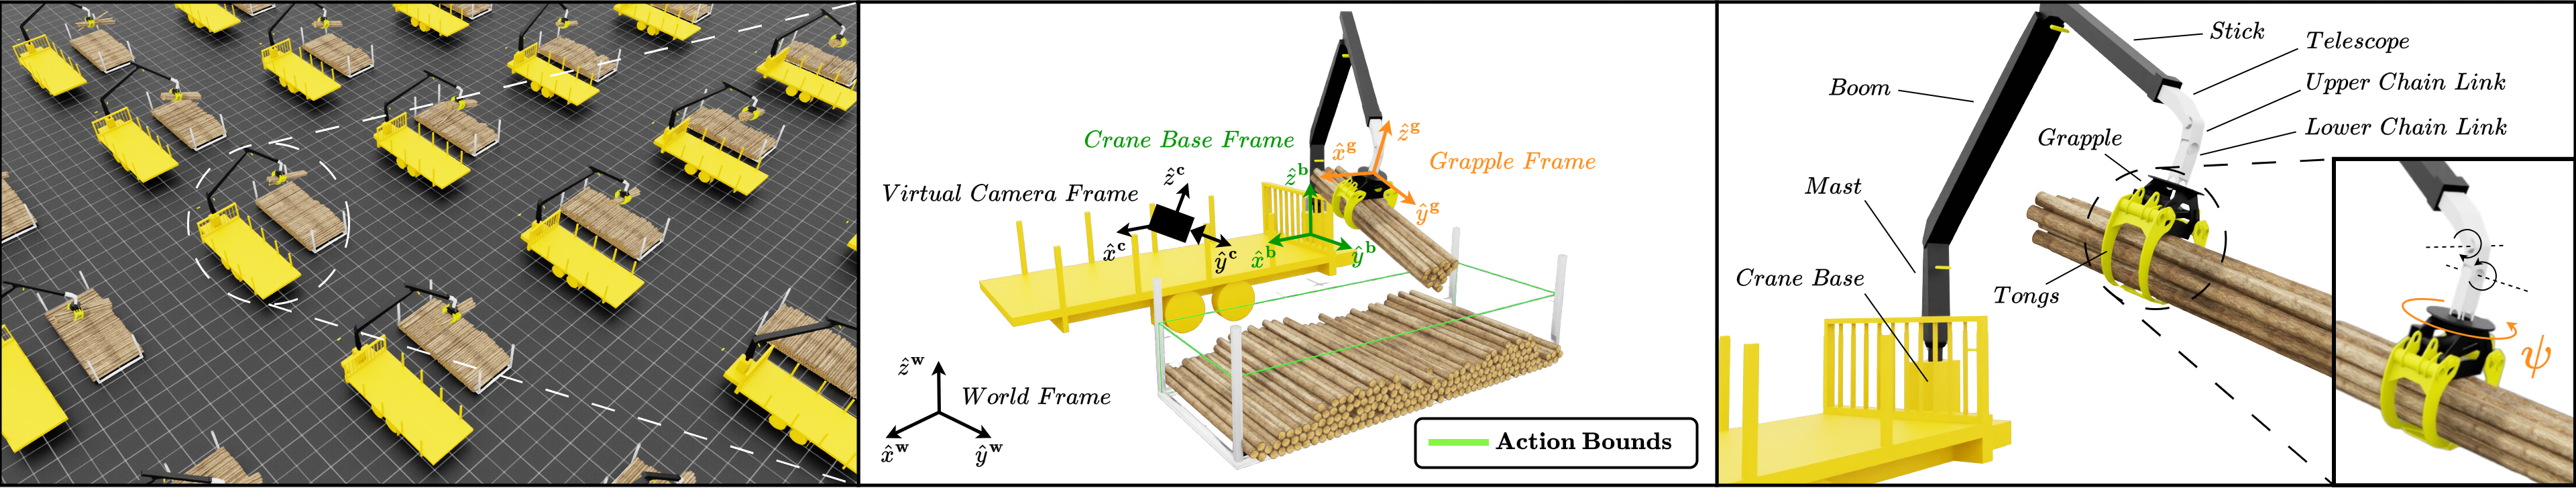
\includegraphics[width=\textwidth]{crane_env.png}                                                                             
\caption{The grasp-and-remove crane environment. From left to right: parallelized training environments in Isaac Sim, each containing
a log loader crane above a rack of 200 logs in randomized configurations; a single environment showing the relevant coordinate frames 
and the action-space bounding box (wireframe); the crane link structure; the passive joints and grapple yaw angle. At each decision
step the policy selects a grasp target within the action bounds, and a finite-state-machine controller executes the pick sequence.}
\label{fig:environment}
\end{figure*}

 \begin{figure}[t]                                                                                                                     
  \centering                                                                                                                          
  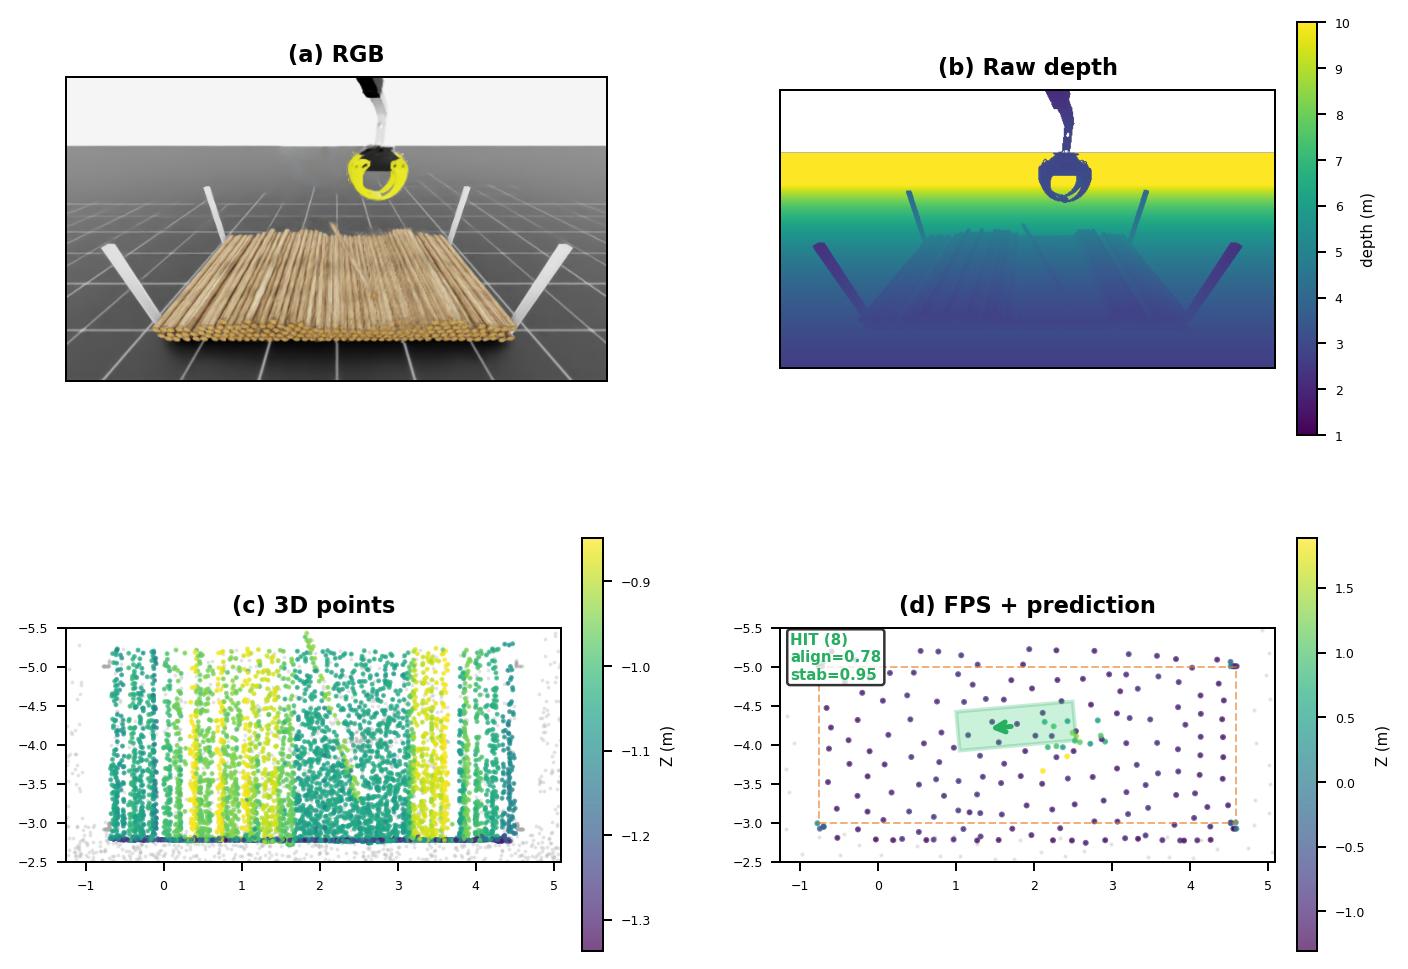
\includegraphics[width=\columnwidth]{episode_001_pipeline_quad_single.png}                                                            
  \caption{Observation pipeline for a single grasp: RGB, raw depth, 3D back-projection in the crane base frame, and FPS-downsampled     
  point cloud with the predicted grasp target and action-space bounds (dashed box).}                                                                 
  \label{fig:pcd_pipeline}                                                                                                            
  \end{figure}


\section{Experiments}
\subsection{Setup}
All experiments share the same crane, rack, and FSM, running on a single NVIDIA RTX 4070 Laptop GPU (8\,GB).
Training uses 32 parallel environments for pose-based policies and 20 for PCD policies (Fig.~\ref{fig:environment}).
Piles contain 200 logs spawned in layered grid patterns; pile variation (Table~\ref{tab:robustness}) randomizes count ($20$--$200$), spacing, offsets, and per-log jitter.
Evaluation runs 100 episodes across 20 parallel environments on identical seeds.
All metrics are per-episode mean $\pm$ std.

\subsection{Metrics}
\label{sec:metrics}
Metrics derived from $(g, \alpha, \varsigma)$ (Section~\ref{sec:outcome}): grasp success rate ($g>0$), throughput (logs per successful grasp), alignment ($\alpha$, grasp-count-weighted), stability ($\varsigma$), pile clearing rate (fraction of logs intentionally removed, excluding knock-offs), and knocked-off percentage.
The clearing progression curve (Fig.~\ref{fig:clearing_curves}) plots fraction cleared vs.\ grasp attempt number.

\section{Results}
\label{sec:results}
\begin{table*}[t]
\centering
\caption{Evaluation results (100 episodes, 200-log piles, mean $\pm$ std). RL uses a symmetric actor-critic; BC$\to$RL uses an asymmetric actor-critic with frozen BC encoder and state-based critic.}
\label{tab:results}
\setlength{\tabcolsep}{5pt}
\begin{tabular}{@{}llcccccc@{}}
\toprule
Method & Obs. & Thru.\,$g$ & Align.\,$\alpha$ & Stab.\,$\varsigma$ & Grasp succ.\,(\%) & Clear rate\,(\%) & Knocked off\,(\%) \\
\midrule
Heuristic & Pose & $\mathbf{9.94 \pm 1.17}$ & $\mathbf{0.918 \pm 0.031}$ & $0.797 \pm 0.018$ & $\mathbf{88.7 \pm 7.8}$ & $99.0 \pm 1.2$ & $1.0 \pm 1.1$ \\
\addlinespace
RL & Pose (128D) & $8.84 \pm 1.68$ & $0.908 \pm 0.040$ & $0.970 \pm 0.021$ & $38.5 \pm 13.5$ & $49.4 \pm 14.8$ & $0.0 \pm 0.2$ \\
RL & Seg.\ PCD   & $7.04 \pm 1.06$ & $0.726 \pm 0.077$ & $0.776 \pm 0.042$ & $53.7 \pm 10.9$ & $55.2 \pm 5.4$ & $0.9 \pm 0.7$ \\
RL & Raw PCD     & $6.78 \pm 1.01$ & $0.758 \pm 0.072$ & $0.815 \pm 0.039$ & $53.3 \pm 8.7$ & $53.0 \pm 3.9$ & $0.6 \pm 0.6$ \\
\addlinespace
BC & Seg.\ PCD   & $9.64 \pm 1.05$ & $0.907 \pm 0.028$ & $0.816 \pm 0.020$ & $70.3 \pm 10.6$ & $96.5 \pm 4.7$ & $0.9 \pm 1.0$ \\
BC & Raw PCD     & $9.32 \pm 1.12$ & $0.904 \pm 0.037$ & $0.824 \pm 0.025$ & $84.5 \pm 9.8$ & $\mathbf{98.5 \pm 5.1}$ & $\mathbf{0.7 \pm 0.7}$ \\
\addlinespace
BC$\to$RL & Raw PCD & $8.65 \pm 0.97$ & $0.906 \pm 0.027$ & $\mathbf{0.947 \pm 0.016}$ & $86.3 \pm 8.5$ & $98.2 \pm 1.5$ & $1.2 \pm 0.8$ \\
\bottomrule
\end{tabular}
\end{table*}

\begin{figure}[t]
\centering
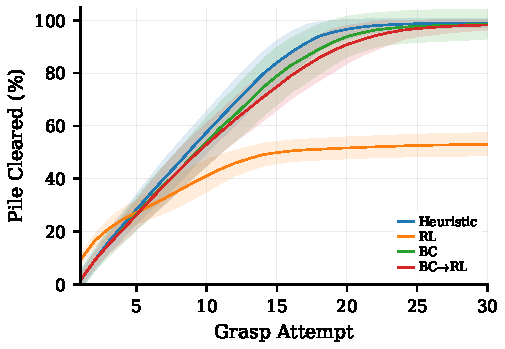
\includegraphics[width=\columnwidth]{clearing_curves.pdf}
\caption{Clearing progression: fraction of 200-log pile cleared vs.\ grasp attempt number (mean $\pm$ std over 100 episodes). RL plateaus at $\sim$53\% while BC, BC+RL, and the heuristic all approach full clearing.}
\label{fig:clearing_curves}
\end{figure}

Table~\ref{tab:results} summarizes evaluation across all methods using the same controller, piles, and protocol.

\subsection{BC+RL Performance}
\label{sec:bcrl_perf}
BC+RL improves grasp stability by 15\% over BC while preserving clearing ability (Table~\ref{tab:results}), surpassing both BC and the privileged-state heuristic in stability.
Alignment remains comparable, so the quality gain is driven entirely by more level lifts.
Throughput is slightly lower, indicating more conservative grasps.

Both the frozen encoder and low noise are critical (Fig.~\ref{fig:bcrl_ablation}): only the frozen-encoder, $\sigma_0 = 0.05$ configuration sustains performance; higher noise or unfreezing the encoder causes collapse.

\begin{figure}[t]
\centering
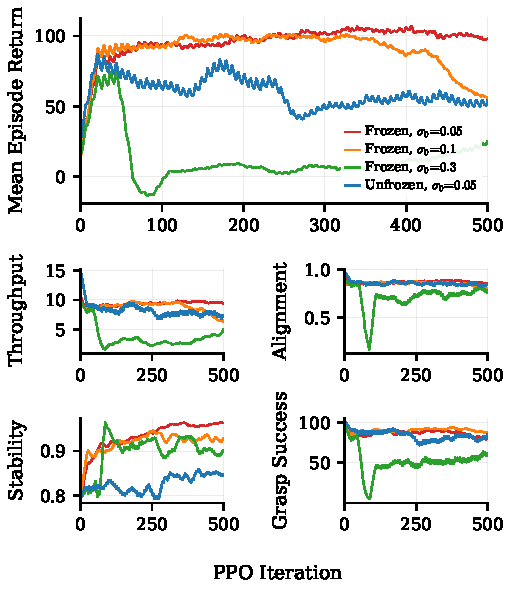
\includegraphics[width=\columnwidth]{bcrl_ablation.pdf}
\caption{BC+RL training sensitivity. Mean episode return vs.\ PPO iteration for four configurations varying encoder freezing and initial policy noise $\sigma_0$. Only the frozen-encoder, low-noise configuration ($\sigma_0 = 0.05$) sustains performance; all other variants collapse during training.}
\label{fig:bcrl_ablation}
\end{figure}

\subsection{BC Performance}
\label{sec:bc_perf}
BC achieves clearing comparable to the heuristic using only raw point clouds (Table~\ref{tab:results}).
Per-grasp metrics closely match the expert; the main gap is in success rate, concentrated in the endgame where sparse logs are harder to localize from depth alone.
For BC, raw PCD outperforms segmented PCD in both clearing and success rate, showing that segmentation provides no benefit.

\subsection{RL Performance}
\label{sec:rl_perf}
From-scratch RL achieves competitive per-grasp reward (Fig.~\ref{fig:reward_curves}) but this does not translate to clearing performance.
Three RL variants (pose, segmented PCD, raw PCD) all plateau at $\sim$53\% clearing (Table~\ref{tab:results}), confirming that RL's failure is fundamental to the exploration landscape rather than an observation limitation.
The policies converge to narrow targeting patterns that work in dense configurations but fail as the pile thins.

\begin{table*}[t]
\centering
\caption{Generalization under pile variation (100 episodes). Each episode samples a random pile: log count in $[20, 200]$, randomized grid dimensions, spacing ($\pm 5$--$15$\%), layer offsets, and per-log jitter.}
\label{tab:robustness}
\setlength{\tabcolsep}{5pt}
\begin{tabular}{@{}llcccccc@{}}
\toprule
Method & Condition & Thru.\,$g$ & Align.\,$\alpha$ & Stab.\,$\varsigma$ & Grasp succ.\,(\%) & Clear rate\,(\%) & Knocked off\,(\%) \\
\midrule
Heuristic & Nominal        & $9.94 \pm 1.17$ & $0.918 \pm 0.031$ & $0.797 \pm 0.018$ & $88.7 \pm 7.8$  & $99.0 \pm 1.2$ & $1.0 \pm 1.1$ \\
Heuristic & Pile variation & $8.28 \pm 1.96$ & $0.889 \pm 0.074$ & $0.789 \pm 0.024$ & $86.3 \pm 11.6$ & $98.2 \pm 4.9$ & $1.3 \pm 1.6$ \\
\addlinespace
BC        & Nominal        & $9.32 \pm 1.12$ & $0.904 \pm 0.037$ & $0.824 \pm 0.025$ & $84.5 \pm 9.8$  & $98.5 \pm 5.1$ & $0.7 \pm 0.7$ \\
BC        & Pile variation & $7.55 \pm 2.02$ & $0.860 \pm 0.093$ & $0.820 \pm 0.029$ & $72.8 \pm 17.7$ & $98.4 \pm 2.5$ & $1.2 \pm 1.5$ \\
\addlinespace
BC$\to$RL & Nominal        & $8.65 \pm 0.97$ & $0.906 \pm 0.027$ & $0.947 \pm 0.016$ & $86.3 \pm 8.5$  & $98.2 \pm 1.5$ & $1.2 \pm 0.8$ \\
BC$\to$RL & Pile variation & $6.97 \pm 1.63$ & $0.861 \pm 0.081$ & $0.922 \pm 0.037$ & $76.0 \pm 14.9$ & $98.5 \pm 1.5$ & $1.3 \pm 1.4$ \\
\bottomrule
\end{tabular}
\end{table*}

\section{Discussion and Limitations}

The clearing progression (Fig.~\ref{fig:clearing_curves}) reveals a divergence around grasp 5--10: RL throughput drops and plateaus near 53\%, while BC, BC+RL, and the heuristic approach full clearing.
Because the per-grasp reward provides no direct incentive for global clearing, RL converges to a narrow targeting pattern that works in dense configurations but fails as the pile thins.
This is not a perception limitation (RL with privileged poses fares no better) but a consequence of the exploration landscape: the policy never discovers the full diversity of pile states encountered during complete clearing.
We also evaluated a throughput-only reward ($r = g$), which achieved comparable per-grasp reward but did not resolve the clearing plateau, further suggesting that the bottleneck is exploration rather than reward design.

BC initialization provides the coverage that RL lacks: demonstrations span the full trajectory from dense stacks to sparse endgames~\cite{rajeswaran2018learning}.
RL fine-tuning optimizes per-grasp quality without rediscovering the targeting strategy.
Freezing the encoder prevents feature drift from the state-based critic (Section~\ref{sec:bcrl}), and low initial noise ($\sigma_0 = 0.05$) prevents overwriting the BC policy.

Raw point clouds match or exceed segmented PCD for both BC and BC+RL (Table~\ref{tab:results}), simplifying the perception pipeline for sim-to-real transfer.
All methods maintain near-complete clearing under pile variation (Table~\ref{tab:robustness}); the learned policies show a larger success-rate drop than the heuristic on varied piles, likely because demonstrations were collected on fixed 200-log configurations.

The grasp-and-remove design has limitations: grasp success is approximated by proximity rather than contact constraints, logs are teleported rather than placed (omitting deposition dynamics), and the PointNet encoder lacks explicit local geometry modeling (e.g., PointNet++~\cite{qi2017pointnetplusplus}).
All experiments are in simulation; sim-to-real transfer is a natural next step.

\section{Conclusion}
We presented a grasp-and-remove crane environment for dense log-pile clearing at scale and compared four methods on a shared evaluation protocol.
From-scratch RL fails regardless of observation type, stalling at $\sim$53\% clearing.
BC from raw point clouds matches the privileged-state heuristic, and BC+RL fine-tuning improves stability by 15\% while maintaining near-complete clearing, demonstrating that demonstrations provide the exploration curriculum RL cannot discover alone.
Future work will explore sim-to-real transfer and richer point cloud architectures.

\section*{ACKNOWLEDGMENT}
[Redacted for anonymity]

\bibliographystyle{IEEEtran}
\bibliography{references}

\end{document}
